\documentclass[handout]{beamer}

%load any additional packages

\usepackage[utf8]{inputenc} % so we can input characters with accents (e.g. ő)

\usepackage{mathtools}

\usepackage{gtbeamer}

\usepackage{graphicx} % ease graphics management
\graphicspath{{images/}} % define folder with images
\usefonttheme{serif} % change font to allow \textbf{}
\usepackage{palatino} % Nicer fonts
\usepackage[ruled]{algorithm2e}
\usepackage{amsmath,amsthm,amssymb} % for math equations
\usepackage{xcolor}
\usepackage{natbib} % richer citation
\usepackage{breakcites} % avoid overfull hbox for long cites

% \theoremstyle{claim}
\newtheorem{claim}[theorem]{Claim}%
\newtheorem{proposition}[theorem]{Proposition}
\setbeamertemplate{footline}[frame number]
\newcommand\norm[1]{\lVert#1\rVert}
% \newcommand\normx[1]{\lVert#1\rVert_{#2}}
\setbeamertemplate{headline}{}

% \usetheme{Szeged}

%% Information (author, title, etc.) %%

\title[PMD]{% short title for footer
    Reinforcement Learning and \\Policy Mirror Descent\\ an introduction
    \vspace{0.5cm}
}

\author{Feiyang Wu}

\institute{
        \textit{College of Computing, School of Computer Science}\\
        \textit{Georgia Institute of Technology}
        \vspace{0.5cm}
}
\date[\today]{
    \today
}

\begin{document}

% Title slide %
{
    \setbeamertemplate{footline}{}
    \setbeamertemplate{headline}{}
    \setbeamercolor{background canvas}{bg=gtblue}
    \maketitle
}

%----------------------------%
% Contents slide
\begin{frame}
\frametitle{Outline}
\tableofcontents
\end{frame}
%----------------------------%

%now include the slides
\setbeamercovered{transparent}
%----------------------------%
\section{Overview}
\begin{frame}{Intro}
    \small
    Suppose you are a robot trying to explore the world. Your decision making process is to optimize your gain from the exploration. Such process can be modelled as a reinforcement learning problem. \\ \vspace{0.5cm}
    The heart of the problem is to \textbf{evaluate} the current situation ("how good am doing right now"), and \textbf{improve} your plan in each situation ("what should be next best move").\\ \vspace{0.5cm}
    Suppose that somehow we come up with an algorithm that can solve all these, how many \textbf{sample} does it need to find a nearly optimal solution?
\end{frame}

\begin{frame}{Intro}
    \small
    Mathematically, we use the following notations,
\begin{itemize}
    \item $\mathcal{S}:$ a set of possible state of the world, for example, a set of every positions on a 2d grid.
    \item $\mathcal{A}$: a set of actions you can take, for example, moving from $(0,0)$ to $(1,1)$.
    \item $p(\cdot|s,a) \in \mathbb{R}$: probability of transitioning to another state when you take action $a$ at state $s$. Notice $\sum_{s'} p(s'|s,a)=1$. This is the so-called \textit{transition kernel}, or transition probability. 
    \item $\pi(a|s)\in \mathbb{R}$: probability of taking action $a\in \mathcal{A}$ given state $s\in \mathcal{S}$; this is the so-called \textit{policy} $\pi: \mathcal{S}\rightarrow \mathcal{A}$. Notice $\sum_{a} \pi(a|s) = 1$.
    \item $r(s,a, s')\in \mathbb{R}$: a real number if you are at state $s$ and take action $a$, and you arrived at state $s'$. 
    \item $s_0, a_0, r_0, s_1, a_1,\cdots$: a sequence of elements termed as a \textit{trajectory}, or the history of samples.
    \item $G_t \coloneqq r_t + \gamma r_{t+1} + \gamma^2 r_{t+2} + \dots = \sum_{k=0}^{\infty} \gamma^{k} r_{t+k}$: the discounted return, note $r_t = r(s_t, a_t)$, and that $G_t = r_t + \gamma G_{t+1}$.
\end{itemize}


\end{frame}

\begin{frame}{Intro}
    At each time step, the agent observes the current state $s$, and subsequently takes an action $a$, which leads to an instantaneous reward $r(s, a, s')$ as well as the transition to the next state according to an unknown transition kernel $p(\cdot | s, a)$. Notice that for each state-action pair, the expected reward is constant, $r(s, a) = \sum_{s'} p(s'|s,a) r(s, a, s')$.
    
    The eventual goal of the agent is to learn a policy to optimize the reward accrued over time. 
\end{frame}

\begin{frame}{Intro}
    \small
    Since the world and the policy is probabilistic, we always consider the expected return. Here we consider the \textbf{expected return} starting at a certain state $s$ and follow policy $\pi$. 
    $$V^{\pi}(s) \coloneqq \mathbb{E}_{\pi} \left[ \sum_{t=0}^{\infty} \gamma^k r_{t} | s_0 = s\right].$$ 
    Another very useful term is the expected return starting at a certain state $s$ but \textbf{take action $a$}, and then follow policy $\pi$. 
    $$Q^{\pi}(s, a) \coloneqq \mathbb{E}_{\pi}\left[G_{t} \mid s_{t}=s, a_{t}=a\right]=\mathbb{E}_{\pi}\left[\sum_{k=0}^{\infty} \gamma^{k} r_{t} \mid s_{0}=s, a_{0}=a\right]$$

\end{frame}

\section{Formulation}
\begin{frame}{Problem formulation}
    \small
    1. Prediction problem:
    \begin{equation*}
        \text{Evaluate } V^{\pi}(s) \quad \forall s\in \mathcal{S}
    \end{equation*}
    2. Control problem:\\
    Define $\Delta_{|\mathcal{A}|}:=\left\{p \in \mathbb{R}^{|\mathcal{A}|} \mid \sum_{i=1}^{|\mathcal{A}|} p_{i}=1, p_{i} \geq 0\right\}, \forall s \in \mathcal{S}$,
    \begin{equation*}
        \begin{aligned}
        \begin{array}{ll}
        \max_{\pi} & \mathbb{E}_{s \sim \nu}\left[V^{\pi}(s)\right] \\
        \text { s.t. } & \pi(\cdot \mid s) \in \Delta_{|\mathcal{A}|}, \forall s \in \mathcal{S} .
        \end{array}
        \end{aligned}
    \end{equation*}
    3. Bound number of sample required to find 
    \begin{equation*}
        \mathbb{E}_{s \sim \nu}\left[V^{\pi}(s)-V^*(s)\right] < \epsilon
    \end{equation*}
    where $\epsilon$ can be any desired accuracy, e.g. $\epsilon = 10^{-3}$, or $\epsilon = 10^{-3} \mathbb{E}_{s \sim \nu}\left[V^*(s)\right]$.
\end{frame}

\begin{frame}{Bellman equation}
    \small
    Let $r_t = r(s_t, a_t, s'_{t+1})$. Given any feasible policy $\pi$, we can expand the value function recursively such that for any time step $t$
    \begin{equation}
    \begin{aligned}
    V^{\pi}(s) & \coloneqq \mathbb{E}_{\pi}\left[G_{t} \mid s_{t}=s\right] \\
    &=\mathbb{E}_{\pi}\left[r_{t}+\gamma r_{t+1} + \gamma^2 r_{t+2} + \cdots \mid s_{t}=s\right] \\
    &=\mathbb{E}_{\pi}\left[r_{t}+\gamma G_{t+1} \mid s_{t}=s\right] \\
    &=\sum_{a} \pi(a | s) \sum_{s^{\prime}} p\left(s^{\prime} \mid s, a\right)\left[r_t +\gamma \mathbb{E}_{\pi}\left[G_{t+1} \mid s_{t+1}=s^{\prime}\right]\right] \\
    &=\sum_{a} \pi(a | s) \sum_{s^{\prime}} p\left(s^{\prime}\mid s, a\right)\left[r_t +\gamma V^{\pi}\left(s^{\prime}\right)\right], \quad \text { for all } s \in \mathcal{S}
\end{aligned}
\end{equation}
We denote this as the Bellman equation. It is also easy to write the Bellman equation for the action-value function.
$$
Q^{\pi}(s,a) = \sum_{s^{\prime}} p\left(s^{\prime}\mid s, a\right)\left[r_t +\gamma V^{\pi}\left(s^{\prime}\right)\right], \quad \text { for all } s \in \mathcal{S}, a\in \mathcal{A}
$$
\end{frame}

\begin{frame}{MDP formulation}
    \small
    \begin{itemize}
        \item Given any policy $\pi$, and some starting state $s_0$, it will generate some state sequence $s_0, s_1, s_2, s_3,\cdots$, which is a discrete time markov process (DTMC).
        \item Markovian property of DTMC: the next state only depends on the last state 
        \item Most of the time we focus on a special kind of DTMC, which is \textit{ergodic}. Such DTMC has a statble distribution $\nu$. 
        \item For ergodic DTMC, whatever is the starting state distribution $s_0 \sim p_0$, it will go to statble distribution $s_t\rightarrow s \sim \nu$.
        \item MDP = DTMC + any feasible policy
        \item \textit{Uniform ergodicity}: assume ergodic DTMC for any policy computed in MDP (usual assumption).
    \end{itemize}
\end{frame}

\begin{frame}{Optimal Policy}
    An \textit{optimal policy} is defined as the policy that has the value function better than or equal to any other value functions of any policies for all states. In other words, $\pi$ is better than $\pi'$ if and only if $V^{\pi}(s) \geq V^{\pi'}(s), \forall s$. There is at least one optimal policy $\pi^*$ (I was told the derivation is highly non trivial, detail is in Siva's notes). Optimal policies share the same value function, the so-called \textit{optimal value function}
    $$
    V^{\pi^*}(s) = \max_{\pi} V^{\pi}(s),$$ and the same \textit{optimal action value function} 
    $$
    Q^{\pi^*} = \max_{\pi} Q^{\pi}(s,a)$$
\end{frame}

\begin{frame}{Optimal value functions}
    The optimal value function and optimal action value function itself satisfy the Bellman equation, together with the fact that the best action for any state is to pick the action with largest $Q$ function, so we have
    \begin{equation}
    \begin{aligned}
    V^{\pi^*}(s) & \coloneqq \max_{a\in\mathcal{A}} Q^{\pi^*}(s,a) \\
    &=\max_{a\in\mathcal{A}} \mathbb{E}_{\pi^*}\left[r_{t}+\gamma G_{t+1} \mid s_{t}=s, a_{t}=a\right] \\
    &=\max_{a\in\mathcal{A}} \mathbb{E}_{\pi^*}\left[r_{t}+\gamma V^{\pi^*}(s_{t+1}) \mid s_{t}=s, a_{t}=a\right] \\
    &=\max_{a\in\mathcal{A}} \sum_{s^{\prime}} p\left(s^{\prime}\mid s, a\right)\left[r_t +\gamma V^{\pi^*}\left(s^{\prime}\right)\right], \quad \text { for all } s \in \mathcal{S}
    \end{aligned}
    \end{equation}
\end{frame}

\begin{frame}{Optimal action value functions}
    Similarly, we have Bellma optimality equation for $Q$ functions,
    \begin{equation}
    \begin{aligned}
    Q^{\pi}(s,a) &= \mathbb{E} \left[r_t +\gamma \max_{a'} Q^{\pi^*}(s_{t+1},a') \mid s_t = s, a_t = a \right] \\
    &= \sum_{s'} p(s'|s,a)\left[ r_t + \gamma \max_{a'} Q^{\pi^*}(s',a') \right]
    \end{aligned}
    \end{equation}
    So far, this concludes contents from Sutton's book up to Chapter 3.
\end{frame}

\begin{frame}{Dynamic Programming}
    From now on, we consider solving the RL/MDP problems starting the prediction problem (evaluate a given policy), and then try to solve the control problem (find a better policy at the same time).
    The first policy evaluation method is the \textit{iterative policy evaluation}. Conside the following update rule,
    \begin{equation}
    \begin{aligned}
    V_{k+1}(s) & \doteq \mathbb{E}_{\pi}\left[R_{t+1}+\gamma V_{k}\left(S_{t+1}\right) \mid S_{t}=s\right] \\
    &=\sum_{a} \pi(a \mid s) \sum_{s^{\prime}} p\left(s^{\prime} \mid s, a\right)\left[r+\gamma V_{k}\left(s^{\prime}\right)\right].
    \end{aligned}
    \end{equation}
    This is essentially treat $V_k$ as the current best estimation of the true value function, and update the estimation using Bellman equation.
\end{frame}

\begin{frame}{Iterative policy evaluation}
Input $\pi$, the policy to be evaluated

Algorithm parameter: a small threshold $\theta>0$ determining accuracy of estimation 

Initialize $V(s)$ arbitrarily, for $s \in \mathcal{S}$, and $V($ terminal $)$ to 0

Loop until $\Delta<\theta$

$\quad \Delta \leftarrow 0$

\quad Loop for each $s \in \mathcal{S}$ :
\begin{equation*}
\begin{aligned}
&v \leftarrow V(s) \\
&V(s) \leftarrow \sum_{a} \pi(a \mid s) \sum_{s^{\prime}} p\left(s^{\prime} \mid s, a\right)\left[r+\gamma V\left(s^{\prime}\right)\right] \\
&\Delta \leftarrow \max (\Delta,|v-V(s)|)
\end{aligned}
\end{equation*}

\end{frame}

\begin{frame}{Policy improvement}
\small
    Suppose you are given a policy $\pi$ and its value functions $V^{\pi}$ and $Q^{\pi}$, we consider the following update rule to find a better policy, guaranteed by policy improvement theorem (not discussed today), 
    \begin{equation*}
    \begin{aligned}
    \pi^{\prime}(s) & \doteq  \arg \max_{a} Q^{\pi}(s, a) \\
    &=\arg \max_{a} \mathbb{E}\left[r_{t}+\gamma V^{\pi}\left(s_{t+1}\right) \mid s_{t}=s, a_{t}=a\right] \\
    &=\arg \max_{a} \sum_{s^{\prime}} p\left(s^{\prime} \mid s, a\right)\left[r+\gamma V^{\pi}\left(s^{\prime}\right)\right]
    \end{aligned}
    \end{equation*}

    The policy found is \textbf{greedy} because we are taking $\max$ from the previous policy. An example of non greedy policy would be, with probability $\epsilon << 1$, we take a random action $a$ with uniformly from the action space, and with $1-\epsilon$ we pick actions according to the greedy policy.
\end{frame}

\begin{frame}{Policy Iteration}
How about we combine them together? Let's introduce \textit{policy iteration}: a single algorithm that performs value iteration and policy improvement at the same time.
\begin{algorithm}[H]
\caption{Policy Iteration}
Initialize $V$ and $\pi$ arbitrarily\;
Loop until $\pi$ stop changing\;
\quad Perform Policy Evaluation\;
\quad Perform Policy Improvement\;
\end{algorithm}
However, such algorithm takes long time to converge, as each step require an policy evaluation step. 
\end{frame}

\begin{frame}{Value Iteration}
\small
    How about we perform one step of Value Iteration and take the newly updated value function for policy improvement, instead of waiting for Value Iteration to converge?

    Consider the following algorithm:
\begin{algorithm}[H]
\caption{Value Iteration}
\While{$\Delta \geq \theta$}{
\For{$s\in \mathcal{S}$}{
$v \leftarrow V(s)$ 

$V(s) \leftarrow \max _{a} \sum_{s^{\prime}} p\left(s^{\prime} \mid s, a\right)\left[r+\gamma V\left(s^{\prime}\right)\right]$

$\Delta \leftarrow \max (\Delta,|v-V(s)|)$
}
}
\end{algorithm}
Notice the difference with the rule from policy evaluation:

\color{red}
$$
V(s) \leftarrow \sum_a \pi(a|s) \sum_{s^{\prime}} p\left(s^{\prime} \mid s, a\right)\left[r+\gamma V\left(s^{\prime}\right)\right]
$$
\end{frame}

\begin{frame}{Asynchronous Algos and GPI}
\small
    So far, all algorithms requires a sweep for all states in a single iteration. This can be computationally trouble if the state space is large and we don't have easy access to all state. Suppose we only have a single trajectory of states $(s_0, s_1, s_2, s_3, \cdots)$. Thus we consider an asynchronous version of algorithms, namely, update $V(s_t)$ whatever $s_t$ is.

\vspace{0.3cm}

    Policy Iteration consists two components, policy iteration and policy evaluation. It turns out that we don't have to wait until policy evaluation to converge completely each time. Sutton coined the process this framework as Generalized Policy Iteration.
    
    \centering
    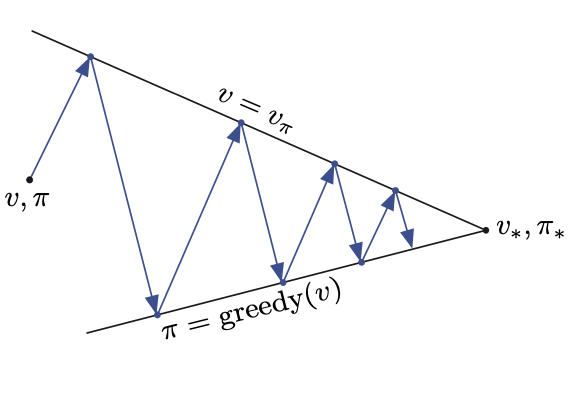
\includegraphics[width=0.4\textwidth]{images/Screenshot 2022-08-10 at 17.16.28.png}
\end{frame}
%----------------------------%
% Conclusions

\section{Summary}
\begin{frame}{Summary }
    \small
    \begin{itemize}
        \item 1
    \end{itemize}
\end{frame}

\begin{frame}
    \frametitle{}
    \centering
    
    \Large\color{gtblue}
    Thank you.

    \vspace{0.5cm}
    feiyangwu@gatech.edu

\end{frame}

%----------------------------%

% References slide
\begin{frame}[allowframebreaks]
\frametitle{References}
\footnotesize
\bibliographystyle{siam}
\bibliography{references} % bibliography file
\end{frame}

%%%%%%%%%%%%%%%%%%%%
\end{document}
%%%%%%%%%%%%%%%%%%%%
